\documentclass[11pt]{article}
\usepackage{amsmath, amssymb, amsthm}
\usepackage[retainorgcmds]{IEEEtrantools}

\usepackage[pdftex]{graphicx}
\usepackage{tikz}
\usetikzlibrary{intersections}

\usepackage{fancyhdr}

%Listings stuff
\usepackage{listings}
\usepackage{lstautogobble}
\usepackage{color}

\definecolor{gray}{rgb}{0.5,0.5,0.5}
\lstset{
basicstyle={\small\ttfamily},
tabsize=3,
numbers=left,
numbersep=5pt,
numberstyle=\tiny\color{gray},
stepnumber=2,
breaklines=true,
boxpos=t
}

%Format stuff
\pagestyle{fancy}
\headheight 35pt

%Header info
\chead{\Large \textbf{Automata and Regex}}
\lhead{}
\rhead{}

\begin{document}
\section{Finite Automata}
	A finite automata is an abstract machine that starts in an initial state, and repeats some task until it ends up in a final state. An automata may have 0 or more end states but only a single start state. When using an automata to implement regex matching, the validity of a string is determined by whether or not the ending state of the automata after parsing is the final state.
	
	It is possible for an automata to have a \textbf{dead state}, that is a non-final state with no possibility of exiting. Most cases these dead states will be omitted from diagrams, so it is safe to assume that any nonexistant edges all lead to a dead state.
	
	\begin{center}
	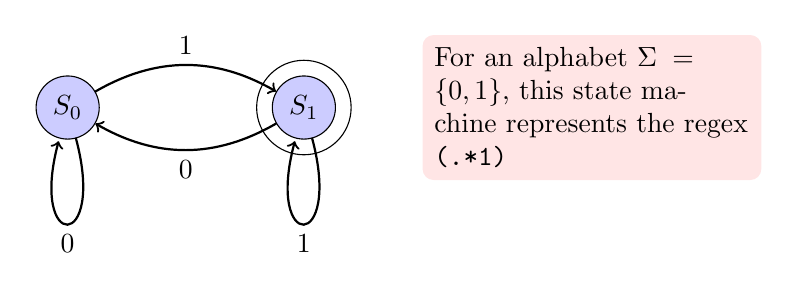
\begin{tikzpicture}
		[scale=3,line cap=round,
		%Styles
		axes/.style=,
		important line/.style={very thick},
		information text/.style={rounded corners,fill=red!10,inner sep=1ex},
		dot/.style={circle,inner sep=1pt,fill,label={#1},name=#1}	,
		main node/.style={circle,fill=blue!20,draw}		
		]
		
		%Colors
		\colorlet{anglecolor}{green!50!black}	%angle arcs/lines
		
		%The graphic
		\node[main node] (S0) at (0,0) {$S_0$};
		\node[main node] (S1) at (1, 0) {$S_1$};
		\draw (1, 0) circle (.2cm);
		
		\path 	(S0)	edge [bend left,->,thick] node[above]{$1$}	(S1)
							edge [loop below,->,thick] node[below]{$0$} (S0)
					(S1)	edge [bend left,->,thick] node[below]{$0$} (S0)
							edge [loop below,->,thick] node[below]{$1$} (S1);
							
		\draw[xshift=1.5cm]
			node[information text,right,text width=4cm] {For an alphabet $\Sigma = \{0,1\}$, this state machine represents the regex \verb|(.*1)|};
	\end{tikzpicture}
	\end{center}
	
\section{Deterministic Finite Automata}
	A DFA cannot have more than one transition leaving a state on the same symbol. A DFA will always produce the exact same path for any given string. A DFA formally is a 5-tuple $(Q, \Sigma, \delta, q_0, F)$.
	\begin{itemize}
		\item $Q$: Finite, non-empty set of states
		\item $\Sigma$: Input alphabet
		\item $\delta$: A transition function $\delta : Q\times \Sigma \rightarrow Q$
		\item $q_0$: A state state $q_0 \in Q$
		\item $F$: A set of final states $F \subset Q$
	\end{itemize}
	
\section{Nondeterministic Finite Automata}
	An NFA can have multiple multiple paths leaving a state encoded with the same symbol. An NFA will yield many possible paths for a given string, and determining the validity of a string requires a backtracking graph search. Formally, an NFA is a 5-tuple $(Q, \Sigma, \Delta, q_0, F)$ with $\Delta : Q \times \Sigma \rightarrow P(Q)$ where $P(Q)$ is the powerset of $Q$.
	
	\subparagraph{NFA-$\epsilon$} An NFA-$\epsilon$ has one or more paths encoded as an empty character, meaning that when reading through string it is possible to take a path without actually advancing a character.
	
\section{Languages}
	A language $L$ is a set of strings defined over an alphabet $\Sigma$ which is a finite set of symbols. There are three operations defined on languages:
	\begin{itemize}
		\item Concatenation: $L_1L_2 = \{xy \mid x \in L_1,  y \in L_2\}$
		\item Union: $L_1 \cup  L_2 = \{x \mid x \in L_1 \text{ or } x \in L_2\}$
		\item Kleene Closure: $L^* = \cup_{i\in N} L^i$, concatenate 0 or more strings from $L$.
	\end{itemize}
	Thus, the language $L^n$, a language consisting of n-length strings, can be built inductively as $LL^{n-1}$.
	
	\subsection{Regular Expressions}
		Regular expressions over $\Sigma$ are representations of languages, and are defined inductively as such:
		\begin{center}
		\begin{tabular}{c|c}
			Regex & Language\\\hline
			$\emptyset$ & $\emptyset$\\
			$\epsilon$ (empty string) & $\{\epsilon\}$\\
			$\forall \sigma \in \Sigma$ & $\{\sigma\}$\\
			$AB$ & $L_AL_B$\\
			$(A|B)$ & $L_A \cup L_B$\\
			$A^*$ & $L_A^*$
		\end{tabular}
		\end{center}
		
\section{NFA Representation of Regex}
	To transform a regex into an NFA (e.g. for a regex engine), define the following two recursive predicates on a regex $e$:
	\begin{itemize}
		\item $e\checkmark$: Holds if $\epsilon \in [[e\checkmark]]$.
		\item $e \xrightarrow{a} e'$: Holds if a string for $e$ can begin with an $a$ and then finish with a string for $e'$.
	\end{itemize}
	
	\subsection{Defining $\checkmark$}
		$\checkmark$ can be defined inductively, given the following rules:
		\begin{itemize}
			\item $\epsilon\checkmark$
			\item $e^*\checkmark$
			\item $e_1\checkmark \implies (e_1 | e_2)\checkmark$
			\item $e_2\checkmark \implies (e_1 | e_2)\checkmark$
			\item $e_1\checkmark \wedge e_2\checkmark \implies (e_1e_2)\checkmark$
		\end{itemize}
		
		\subparagraph{Goal-Directed Proof} To prove $\checkmark$, start with the premise to prove, and work backwards. Applicable rules for a given conclusion are determined by the top-most operator in the expression, generating sub-goals until you reach axioms everywhere or you get stuck.
		
		\subparagraph{Algorithm} Straightforward, goal-directed recursive algorithm.
		\begin{lstlisting}[autogobble=true,mathescape]
			def check(e):
				switch e:
					case a, None: return False
					case $\epsilon$, f*: return true
					case e_1 | e_2:
						return check(e_1) or check(e_2)
					case e_1e_2:
						return check(e_1) and check(e_2)
		\end{lstlisting}
		
	\subsection{Defining $\xrightarrow{a}$}
		Like $\checkmark$, $\xrightarrow{a}$ is defined inductively using a set of rules. The key intuition is that $e\xrightarrow{a} e'$ means that strings for $e$ can begin with an a and then finish with a string that matches $e'$.
		\begin{itemize}
			\item $a \xrightarrow{a} \epsilon$
			\item $e_1 \xrightarrow{a} e'_1 \implies e_1|e_2 \xrightarrow{a} e'_1$
			\item $e_2 \xrightarrow{a} e'_2 \implies e_1|e_2 \xrightarrow{a} e'_2$
			\item $e_1 \xrightarrow{a} e'_1 \implies e_1e_2 \xrightarrow{a} e'_1e_2$
			\item $e_1\checkmark \wedge e_2 \xrightarrow{a} e'_2 \implies e_1e_2 \xrightarrow{a} e'_2$
			\item $e \xrightarrow{a} e' \implies e^* \xrightarrow{a} e'e^*$
		\end{itemize}
		\subparagraph{Algorithm} The algorithm for this definition is a little less straightforward than the algorithm for checks.
		\begin{lstlisting}[autogobble=true,mathescape]
			def trans(e):
				switch e:
					case None, $\epsilon$: return {}
					case a: return {<a, $\epsilon$>}
					case e_1|e_2:
						return trans(e_1) $\cup$ trans(e_2)
					case e_1e_2:
						s = trans(e_2) if check(e_1) else {}
						return ({<a,e'e_2> if <a,e'> in trans(e_1)} $\cup$ s)
					case f*:
						return ({<a,f'f*> if <a,f'> in trans(f)})
		\end{lstlisting}
		
	\subsection{Algorithm}
		Given a regex $e$, the NFA of e, $<e>$, is defined as the following tuple:
		\begin{itemize}
			\item States: RE's reachable from $e$ via $\xrightarrow{a}$ sequences
			\item Start state: $e$
			\item Transitions: $\xrightarrow{a}$
			\item Final States: $\checkmark$
		\end{itemize}
		
		\begin{lstlisting}[autogobble=true,mathescape]
			def reduce(e):
				$\delta$, $\Sigma$ = {}		# Initialize transitions, alphabet
				Q = N = {e}		# Initialize state sets
				q_0 = e		# Create initial state
				
				while N != {}:		# Until no states need processing
					choose d in N
					N -= {d}
					if check(d):
						F += {d}	# Final state
					for <a,d'> in trans(d):	# Compute transitions
						if d' not in Q:		# New target
							Q += {d'}
							N += {d'}
						$\Sigma$ += {a}
						$\delta$ += {<d, a, d'>}		# Update transition
				return <$\Sigma$, Q, q_0, F, $\delta$>
		\end{lstlisting}
%	\begin{center}
%	\begin{tikzpicture}
%		[scale=3,line cap=round,
%		%Styles
%		axes/.style=,
%		important line/.style={very thick},
%		information text/.style={rounded corners,fill=red!10,inner sep=1ex},
%		dot/.style={circle,inner sep=1pt,fill,label={#1},name=#1}			
%		]
%		
%		%Colors
%		\colorlet{anglecolor}{green!50!black}	%angle arcs/lines
%		
%		%The graphic
%	\end{tikzpicture}
%	\end{center}

%	\begin{figure}[htb]
%		\centering
%		\includegraphics[width=0.8\textwidth]{filename.eps}
%		\caption{Caption.}
%		\label{fig:figure}
%	\end{figure}

%		\def\enotesize{\normalsize}
%		\theendnotes
\end{document}